\documentclass{article}

\usepackage{amsmath,amssymb,amsthm,textcomp,mathtools}

\usepackage{tikz}
\usepackage{pgfplots}
\pgfplotsset{compat=1.18}

\title{On Math}
\author{Jacek Walczak}
\date{February - March 2025}

\begin{document}

\maketitle

\section{General notes and todos}
- I feel like multiline equations should have higher vertical spacing
- Trigonometry values can be done in a single table

\section{Default symbols}

A - area

\section{Trigonometry}

\begin{equation}
  \begin{gathered}
    \sin\theta = \frac{\text{opposite}}{\text{hypotenuse}} \\
    \cos\theta = \frac{\text{adjacent}}{\text{hypotenuse}} \\
    \tan\theta = \frac{\text{opposite}}{\text{adjacent}} \\
    \csc\theta = \frac{1}{\sin{\theta}} =
    \frac{\text{hypotenuse}}{\text{opposite}} \\
    \sec\theta = \frac{1}{\cos{\theta}} =
    \frac{\text{hypotenuse}}{\text{adjacent}} \\
    \cot\theta = \frac{1}{\tan{\theta}} =
    \frac{\text{adjacent}}{\text{opposite}} \\
  \end{gathered}
\end{equation}

\subsection{Sine values}
\begin{equation}
  \begin{gathered}
    \sin(0) = 0 \\
    \sin(30) = \frac{1}{2} \\
    \sin(45) = \frac{\sqrt{2}}{2} \\
    \sin(60) = \frac{\sqrt{3}}{2} \\
    \sin(90) = 1
  \end{gathered}
\end{equation}

\subsection{Cosine values}
\begin{equation}
  \begin{gathered}
    \cos(0) = 1 \\
    \cos(30) = \frac{\sqrt{3}}{2} \\
    \cos(45) = \frac{\sqrt{2}}{2} \\
    \cos(60) = \frac{1}{2} \\
    \cos(90) = 0
  \end{gathered}
\end{equation}

% Tangent values

\subsection{Tangent values}
\begin{equation}
  \begin{gathered}
    \tan(0) = 0 \\
    \tan(30) = \frac{1}{\sqrt{3}} = \frac{\sqrt{3}}{3} \\
    \tan(45) = 1 \\
    \tan(60) = \sqrt{3} \\
    \tan(90) = \text{undefined}
  \end{gathered}
\end{equation}

\subsection{Formula of a general triangle}

\begin{equation}
  A = \frac{1}{2}ab \sin{C}
\end{equation}
where \textit{C} is the measure of the angle between sides \textit{a} and \textit{b} (also called \textit{included angle})

\subsection{Law of sines}
% TODO: image needed

\begin{equation}
  \frac{a}{\sin A} = \frac{b}{\sin B} = \frac{c}{\sin C}
\end{equation}
and also:
\begin{equation}
  \frac{\sin A}{a} = \frac{\sin B}{b} = \frac{\sin C}{c}
\end{equation}
When we have obtuse angle we need to subtract the result from $180$.


\section{Complex numbers}
Complex numbers can be represented by the point $(x, y)$ where $x$ is real axis and $y$
is imaginary axis. We call this plane as a \textbf{complex plane}, also called
\textit{Argand diagram}, denoted as $C$.

\subsection{Powers of $i$}
\begin{equation}
  \begin{gathered}
    i^1 = \sqrt{-1} \\
    i^2 = (\sqrt{-1})^2 = -1 \\
    i^3 = -1 * i = -i \\
    i^4 = (-1) * (-1) = 1
  \end{gathered}
\end{equation}
and so on...

\subsection{Magnitude of a complex number}
The magnitude of a complex number is its distance from the origin $(0, 0)$.
It is denoted az $|z|$. For complex number $z = a + bi$ magnitude is:
\begin{equation}
  |z| = \sqrt{a^2 + b^2}
\end{equation}

\subsection{Argument of a complex number}
There is natural angle $\theta$ that \textit{z} makes with real x-axis. This angle is called \textit{the argument of z}. The numeric value of $arg(z)$ is given in radians and also
\begin{equation}
0 \leq arg(z) \leq 2\pi
\end{equation}
Example:
\begin{equation}
  \begin{gathered}
  z = 3 + 4i \\
  \tan \theta = \frac{4}{3} \\
  \theta = \arctan\frac{4}{3} \approx 0.93
  \end{gathered}
\end{equation}

\section{Geometry}
\subsection{Rigid motions}
Or sometimes - any transformations that does not change the distances
and angles between points in a figure. They are \textbf{angle-preserving} and
\textbf{distance-preserving}.


Rigid motions types:

- translations

- rotations

- reflections


Not a rigid motions:

- dilations

- stretches

\section{Displacement}
\begin{equation}
  s = ut+\frac{1}{2}gt^2
\end{equation}
where:

$s$ - displacement of the object measured in meters

$u$ - initial velocity of the object measured in meters per second

$t$ - time measured in seconds

$g$ - $9.8\frac{m}{s^2}$ - constant acceleration due to gravity
\section{Functions}
\subsection{Standard form}
\begin{equation}
  ax + by = c
\end{equation}
\subsection{Parallel lines}
Calculate equation of the parallel line:
\begin{equation}
  y - y_1 = m(x - x_1)
\end{equation}
Calculate a slope of a line given two points:
\begin{equation}
  m = \frac{y_2 - y_1}{x_2 - x_1}
\end{equation}
\subsection{Quadratic formula}
\begin{equation}
  x = \frac{-b \pm \sqrt{b^2 - 4ac}}{2a}
\end{equation}

\subsection{Odd and even functions}
Function is said to be odd if:
\begin{equation}
  f(-x) = -f(x)
\end{equation}
Function is said to be even if:
\begin{equation}
  f(-x) = f(x)
\end{equation}
\subsection{Factor cubics by grouping}
For example to factor following function by grouping:

\begin{equation}
  3x^3-6x^2+2x-4
\end{equation}
1. group them
\begin{equation}
  (3x^3-6x^2)+(2x-4)
\end{equation}
2. factor larger terms so the leftover match
\begin{equation}
  3x^2(x-2)+2(x-2)
\end{equation}
3. factor out the binomial
\begin{equation}
  (3x^2+2)(x-2)
\end{equation}
Note: not all cubics can be factored, however,
of the cubics that can be factored,
many can be factored by grouping

\subsection{Factor theorem}
For polynomial, if we know root, we can determine a factor of the
polynomial. If $p(x)$ is a polynomial and $x=r$ is a root of $p(x)$ then
\begin{equation}
  p(r) = 0
\end{equation}
so $(x-r)$ is a factor of $p(x)$
generally: $(ax-b)$ is a factor of a polynomial $p(x)$ then:
\begin{equation}
  x = \frac{b}{a} is a root of p(x)
\end{equation}

\subsection{Rational roots theorem}
Support the rational number $\frac{p}{q}$ in lowest terms, is a root of a polynomial
with integer coefficient.
% TODO: add colors to differentiate
Then 'p' must be the factor of the polynomial's constant term, and 'q' must be a factor
of its leading coefficient.
Given a polynomial with integer coefficient, any rational roots of the polynomial must take the
form:
\begin{equation}
  \pm \frac{factor  of  the  constant  term}{factor  of  the  leading  coefficient}
\end{equation}
For example:
\begin{equation}
  f(x) = 8x^3 + 12x^2 + 6x + 2
\end{equation}
so we have 16 possible roots:
\begin{equation}
  \begin{gathered}
    % TODO: strike through
    \pm \frac{1}{1}, \pm \frac{1}{2}, \pm \frac{1}{4}, \pm \frac{1}{8}, \\
    \pm \frac{2}{1}, \pm \frac{2}{2}, \pm \frac{2}{4}, \pm \frac{2}{8}
  \end{gathered}
\end{equation}
Removing the duplicates, we have 10 possible rational roots:
\begin{equation}
  \pm \frac{1}{8}, \pm \frac{1}{4}, \pm \frac{1}{2}, \pm 1, \pm 2
\end{equation}
Note: it is about \textbf{possible} rational roots.

\subsection{Function composition}
\begin{equation}
  (f \circ g)(x) = f(g(x))
\end{equation}
\subsection{Inverse functions}
Inverse functions are denoted by $f^{-1}(x)$.
For $f(x)$ that maps $x=2$ to $y=0$ an inverse function $f^{-1}(x)$ instantiation would be
$f^{-1}(0)=0$.
Generally it is a simple composition:
\begin{equation}
  f^{-1}(f(x)) = x
\end{equation}
so
\begin{equation}
  (f^{-1} \circ f)(x) = x
\end{equation}


Calculate inverse function:
1. swap $x$ and $y$

2. solve for $y$

Example:
\begin{equation}
  \begin{gathered}
    f(x) = 3x-9 \\
    y = 3x-9 \\
    x = 3y-9 \\
    x-3y=-9 \\
    x+9=3y \\
    \frac{x+9}{3}=y \\
    f^{-1}(x)=\frac{x+9}{3}
  \end{gathered}
\end{equation}

Domain of a function $f(x)$ is the range of its inverse function $f^{-1}(x)$.

Range of a function $f(x)$ is the domain of its inverse function $f^{-1}(x)$.

\subsection{Multiplicities of the roots of a polynomial}
\begin{equation}
  p(x) = (x-5)^2(x+8)
\end{equation}
for that polynomial roots are $x=5$ and $x=-8$ but factor $(x-5)^2$
appears \textbf{twice} so it is a \textbf{multiple root}
$(x+8)$ on the other hand is a \textbf{simple root}.

\subsection{Intersection of a reciprocal function and a straight line}
There are three possibilities when considering the intersection of a reciprocal
function and a straight line:
1. there are two intersection points
2. there is only one intersection point
3. there are no intersection points at all

% TODO: needs images

Typically, when computing the points of intersection of a reciprocal
function and a line, we have to solve a system of two equations.

% TODO: needs bracket over two first lines
\begin{equation}
  \begin{gathered}
    y = x \\
    y = \frac{1}{x} \\
    x = \frac{1}{x} \\
    x^2 = 1 \\
    x = \pm 1
  \end{gathered}
\end{equation}

\subsection{Rational functions}
Horizontal asymptotes

1. Identify the 'dominant term' which is a leading term of the polynomial though we
usually ugnore the coefficients.

2. Divide every term in the numerator and denominator of $f(x)$ by the dominant term.

3. Evaluate the remaining expression as $x \to \infty$.


Roots


\subsection{Radical function}
Range of a radical function $f(x) = \sqrt[n]{x}$ depends on index \textit{n} whether it's even or odd.

For odd index like in function $f(x) = -2\sqrt[3]{3x-2}+2$ range is $(-\infty, \infty)$.
Transformations do not change its range.

For even index $n$ range is $x \geqslant 0$ but the transformations can change the range.
Horizontal shifts and stretches doesn't change the the range.

For example for function $g(x) = -3\sqrt[4]{2x-1}-2$:
\begin{equation}
  \begin{gathered}
  \sqrt[4]{2x-1} \geqslant 0 \\
  -3\sqrt[4]{2x-1} \leqslant 0 \\
  -3\sqrt[4]{2x-1} \leqslant -2 \\
  g(x) \leqslant -2
  \end{gathered}
\end{equation}

\subsection{Reciprocal functions}

\begin{figure}
\centering
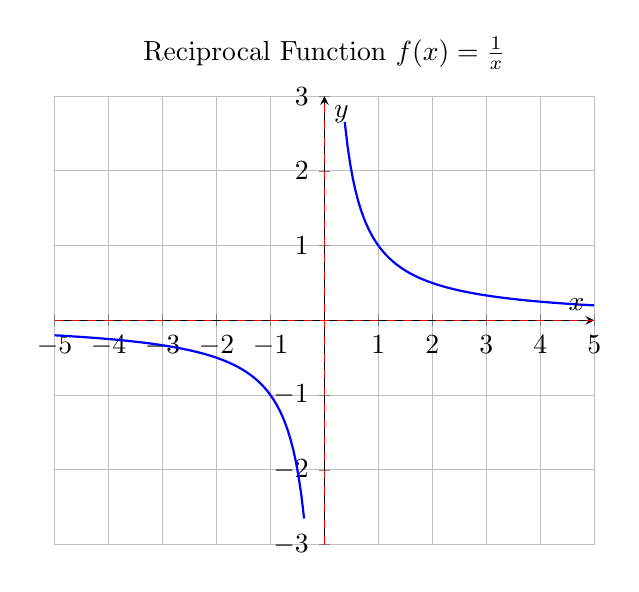
\begin{tikzpicture}
\begin{axis}[
    axis lines=center,
    xlabel=$x$,
    ylabel=$y$,
    title={Reciprocal Function $f(x) = \frac{1}{x}$},
    xmin=-5, xmax=5,
    ymin=-3, ymax=3,
    xtick={-5,-4,-3,-2,-1,1,2,3,4,5},
    ytick={-3,-2,-1,1,2,3},
    grid=both,
    domain=-5:5,
    samples=200,
    restrict y to domain=-3:3,
]
% Plot the function, excluding the region around x=0
\addplot[blue, thick] {1/x};

% Add asymptotes
\draw[dashed, red] (axis cs:0,-3) -- (axis cs:0,3);
\draw[dashed, red] (axis cs:-5,0) -- (axis cs:5,0);
\end{axis}
\end{tikzpicture}
\caption{Graph of the reciprocal function $f(x) = \frac{1}{x}$}
\end{figure}


%TODO: image
\begin{equation}
  f(x) = \frac{1}{x}
\end{equation}
When function is not transformed, it passes through points $(-1, -1)$ and $(1, 1)$.
% TODO: not range?
Domain of (transformed) reciprocal function
\begin{equation}
f(x) = \frac{a}{bx+c} + d
\end{equation}
has the horizontal asymptote $y = d$ therefore the range is
\begin{equation}
f(x) = \in (-\infty, d) \cup (d, \infty)
\end{equation}
% TODO: range
Range of (transformed) reciprocal function
\begin{equation}
f(x) = \frac{a}{bx+c} + d
\end{equation}
has the vertical asymptote $y = d$ therefore the range is
\begin{equation}
f(x) = \in (-\infty, d) \cup (d, \infty)
\end{equation}


\subsection{Exponential functions}
\subsection{Logarithmic functions}
\section{Statistics}
\subsection{Estimating a mean and variance}
\subsection{Sum of squares}
\subsection{Linear coefficient}
Signed with $\rho$ (Greek letter called 'rho').
- $\rho = 1$ means perfect positive correlation
- $\rho = -1$ means perfect negative correlation
- $\rho = 0$ no (linear) correlation
\section{Logarithms}
\begin{table}[htbp]
\centering
\begin{tabular}{|l|l|}
\hline
\textbf{Property} & \textbf{Formula} \\
\hline
Product Rule & $\log_a(xy) = \log_a(x) + \log_a(y)$ \\
\hline
Quotient Rule & $\log_a\left(\frac{x}{y}\right) = \log_a(x) - \log_a(y)$ \\
\hline
Power Rule & $\log_a(x^n) = n \cdot \log_a(x)$ \\
\hline
Change of Base & $\log_a(x) = \frac{\log_b(x)}{\log_b(a)}$ \\
\hline
Equating arguments & $\log_af(x) = log_ag(x)$ is the same as $f(x) = g(x)$ \\
\hline
\end{tabular}
\caption{Fundamental Properties of Logarithms}
\label{tab:log_properties}
\end{table}

% Approach 1: Looser Table with More Spacing
\begin{table}[htbp]
\centering
\renewcommand{\arraystretch}{1.5} % Increases vertical spacing between rows
\setlength{\tabcolsep}{15pt} % Increases horizontal spacing between columns
\begin{tabular}{|l|p{5cm}|p{6cm}|}
\hline
\textbf{Property} & \textbf{Formula} & \textbf{Description} \\
\hline
\textbf{Product Rule} &
$\log_a(xy) = \log_a(x) + \log_a(y)$ &
The logarithm of a product equals the sum of the individual logarithms. This transforms multiplication into addition. \\
\hline
\textbf{Quotient Rule} &
$\log_a\left(\frac{x}{y}\right) = \log_a(x) - \log_a(y)$ &
The logarithm of a quotient equals the difference of logarithms. This transforms division into subtraction. \\
\hline
\textbf{Power Rule} &
$\log_a(x^n) = n \cdot \log_a(x)$ &
The logarithm of a value raised to a power equals the power multiplied by the logarithm. This transforms exponentiation into multiplication. \\
\hline
\textbf{Change of Base} &
$\log_a(x) = \frac{\log_b(x)}{\log_b(a)}$ &
This formula allows conversion between different logarithmic bases, useful when calculating logarithms with bases other than those built into calculators. \\
\hline
\end{tabular}
\caption{Fundamental Properties of Logarithms}
\label{tab:log_properties}
\end{table}

% Approach 2: List Format with Titles for Each Property
\section*{Logarithmic Properties}

\subsection*{Product Rule}
\begin{equation}
\log_a(xy) = \log_a(x) + \log_a(y)
\end{equation}

The product rule allows us to express the logarithm of a product as the sum of logarithms. This is one of the fundamental properties that makes logarithms powerful for simplifying complex calculations. When we take the logarithm of a product of two numbers, we can break it down into the sum of the logarithms of each number.

\subsection*{Quotient Rule}
\begin{equation}
\log_a\left(\frac{x}{y}\right) = \log_a(x) - \log_a(y)
\end{equation}

The quotient rule states that the logarithm of a quotient equals the logarithm of the numerator minus the logarithm of the denominator. This property transforms division operations into subtraction of logarithms, which is often easier to work with.

\subsection*{Power Rule}
\begin{equation}
\log_a(x^n) = n \cdot \log_a(x)
\end{equation}

The power rule tells us that the logarithm of a number raised to a power equals the power multiplied by the logarithm of the number. This property is especially useful when dealing with expressions containing exponents, as it converts exponentiation to multiplication.

\subsection*{Change of Base Formula}
\begin{equation}
\log_a(x) = \frac{\log_b(x)}{\log_b(a)}
\end{equation}

The change of base formula allows us to convert logarithms from one base to another. This is particularly useful in practical applications since most calculators only directly compute natural logarithms (base $e$) and common logarithms (base 10). Using this formula, we can express logarithms of any base in terms of logarithms of a different base.

\section{Finite sequences}
Coefficient rule:
\begin{equation}
  \sum_{i=1}^{n} ca_i = c * \sum_{i=1}^{n} a_i
\end{equation}

Sum rule:
\begin{equation}
  \sum_{i=1}^{n} (a_i+b_i) = \sum_{i=1}^{n} a_i + \sum_{i=1}^{n} b_i
\end{equation}

\section{Polynomial identities}
\begin{flalign*}
& (a + b)^2 = a^2 + 2ab + b^2 & \\
& (a - b)^2 = a^2 - 2ab + b^2 & \\
& (a + b)^3 = a^3 + 3a^2b + 3ab^2 + b^3 & \\
& (a - b)^3 = a^3 - 3a^2b + 3ab^2 - b^3 & \\
& a^2 - b^2 = (a + b)(a - b) & \\
& a^3 - b^3 = (a - b)(a^2 + ab + b^2) & \\
& a^3 + b^3 = (a + b)(a^2 - ab + b^2) &
\end{flalign*}

\section{Derivatives}
Average rate of change of the function $f(x)$ on the interval $[a, a+h]$:

\begin{equation}
  \frac{\Delta y}{\Delta x} = \frac{f(a+h) - f(a)}{h}
\end{equation}

Instanteous rate of change of the function at the point $x=a$ is the limit of the average
rate of change as $h \rightarrow 0$. It's denoted by $f'(a)$ and given by:

\begin{equation}
  f'(a) = \lim_{h \rightarrow 0}\frac{f(a+h) - f(a)}{h}
\end{equation}

and its value is equal to the slope of the tangent line to the curve $y = f(x)$ at $x=a$.
Also it can be defined as:
\begin{equation}
  f'(a) = \lim_{x \rightarrow a}\frac{f(x) - f(a)}{x-a}
\end{equation}

\subsection{Differentiation of an exponent function}
\begin{equation}
  \frac{d}{dx} (a^x) = a^x\ln a
\end{equation}
with special case:
\begin{equation}
  \frac{d}{dx} (e^x) = e^x\ln e = e^x * 1 = e^x
\end{equation}
\subsection{Chain rule for exponent function}
\begin{equation}
  \begin{gathered}
    y = e^{3x} \\
    y = e^u \\
    u = 3x \\
    \frac{dy}{dx} = \frac{dy}{du} * \frac{du}{dx} \\
    \frac{d}{du} e^u = e^u \\
    \frac{d}{dx} 3x = 3 \\
    \frac{dy}{dx} = e^u * 3 = 3e^u = 3e^{3x}
  \end{gathered}
\end{equation}

\subsection{Derivative of the (natural) logarithm}
For natural logarithm:
\begin{equation}
  \frac{d}{dx}(\ln x) = \frac{1}{x}
\end{equation}
For general logarithm:
\begin{equation}
  \frac{d}{dx}(\log_a x) = \frac{1}{x\ln a}
\end{equation}
Example with changing base:
\begin{equation}
  \begin{gathered}
  \log_ax = \frac{\ln x}{\ln a} \\
  \frac{d}{dx}(\log_ax) = \frac{d}{dx}(\frac{\ln x}{\ln a}) = \\
  = \frac{1}{\ln a} * \frac{d}{dx}(\ln x) = \\
  = \frac{1}{\ln a} * \frac{1}{x} = \frac{1}{x\ln a}
  \end{gathered}
\end{equation}
\subsection{Chain rule for logarithmic function}
\begin{equation}
  \begin{gathered}
  y = \ln(2x+1) \\
  y = \ln u \\
  u = 2x+1 \\
  y' = \frac{1}{u} \\
  u' = 2 \\
  \frac{dy}{dx} = \frac{1}{u} * 2 = \frac{2}{u} = \frac{2}{2x+1}
  \end{gathered}
\end{equation}

\section{Integrals}
Also called \textit{antiderivatives}. To represent integrals we use an integral
symbol. For example:
\begin{equation}
  \int 2x dx = x^2 + C
\end{equation}
Integrals like this are called 'indefinite integrals' and (in this case)
function being integrated is called an 'integrand'.

\subsection{Integral of a sum of functions}
\begin{equation}
  \int f(x) \pm g(x) \, dx = \int f(x) \, dx \pm \int g(x) \, dx
\end{equation}

\subsection{Integral of a reciprocal function}
\begin{equation}
  \int \frac{1}{x} \, dx = \int \ln abs(x) + C
\end{equation}
and also:
\begin{equation}
  \int \frac{1}{x} \, dx = \int \ln|x| + C = \ln abs(x) + \ln K = \ln (K (abs(x))
\end{equation}

\subsection{Integral of an exponential function}
\begin{equation}
  \int e^x \, dx = e^x + C
\end{equation}
with general base we know that
\begin{equation}
  \frac{d}{dx} (a^x) = a^x \ln a
\end{equation}
so reversing:
\begin{equation}
  \int a^x \, dx = \frac{a^x}{\ln a} + C
\end{equation}

\subsection{Power rule for differentiation in reverse}
\begin{equation}
  \frac{d}{dx}(x^{n+1}) = (n+1)x^n
\end{equation}
same as:
\begin{equation}
  \int x^ndx = \frac{x^{n+1}}{n+1}
\end{equation}
Note: power rule does not work if $n=-1$!

\section{Sandbox}
Marked integral for future
\begin{equation}
  \int_{a}^{b} f(x) \, dx
\end{equation}

\end{document}
